\section{Interleaved Practice}
Wir stellen uns vor, dass zwei Themen unterrichtet werden sollen, Thema A und Thema B.
Das Naheliegendste wäre nun, zuerst mehrere Lektionen ausschliesslich zum Thema A zu unterrichten.
Wenn dieses Thema abgeschlossen ist, wir werden mehrere Lektionen zum Thema B unterrichtet.
Diesen Ansatz nennen wir \textit{blocked study}~\cite{Carvalho2014}.
Im Gegensatz dazu steht der Ausdruck \textit{interleaved study}~\cite{Carvalho2014}.
Damit ist gemeint, dass die Themen A und B jeweils abwechslungsweise unterrichtet werden.
Symbolisch schreiben wir dafür
\begin{itemize}
	\item blocked: AAAABBBB
	\item interleaved: ABABABAB
\end{itemize}
Diese Begriffe können sich auch auf die Reihenfolge von Übungsaufgaben beziehen anstatt auf die Reihenfolge von Unterrichtsblöcken.
Wir nennen das entsprechend \textit{blocked practice} und \textit{interleaved practice}.

Generell scheint der Ansatz \glqq{}interleaved\grqq{} langfristig besseren Lernerfolg zu versprechen als \glqq{}blocked\grqq{}.
Für den Mathematikunterricht wurde dies zum Beispiel durch Rohrer und Taylor untersucht in \cite{Rohrer2007}.
Dabei wurden zwei Experimente durchgeführt, von denen wir hier das zweite kurz zusammenfassen.
Die Lernenden in zwei Gruppen aufgeteilt.
Eine lernte nach dem \glqq{}interleaved\grqq{} Prinzip, die andere nach dem \glqq{}blocked\grqq{}.
Dabei ging es um Volumenberechnungen dreidimensionaler Körper, genauer um Zylinder, Kugeln, Spheroid und Kegel.
Die verschiedenen Themen entsprechen genau diesen vier Klassen von Körpern.
Beide Gruppen erhielten den selben Unterricht und die selben Aufgaben.
Die \glqq{}blocked\grqq{}-Gruppe löste allerdings alle Aufgaben zur selben Körperklasse hintereinander, währen die Aufgaben beider \glqq{}interleaved\grqq{}-Gruppe gemischt waren.
Während der Übungsaufgaben schnitt die \glqq{}blocked\grqq{}-Gruppe besser ab.
Doch beim anschliessenden Test, der gemischte Aufgaben enthielt, schnitt die \glqq{}interleaved\grqq{}-Gruppe deutlich besser ab.
Dies ist in Abbildung~\ref{fig:interleaved} gezeigt.

\begin{figure}[ht]
	\centering
	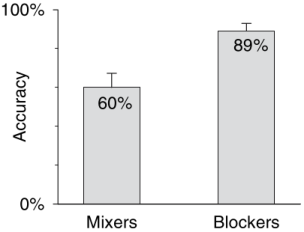
\includegraphics[width=0.4\textwidth]{images/interleaved_practice}
	\hfill
	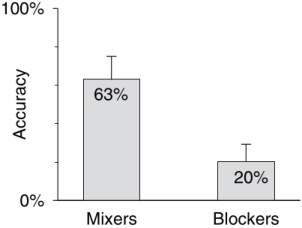
\includegraphics[width=0.4\textwidth]{images/interleaved_test}
	\caption{Resultate bei den Übungen (links) und den Test (rechts)~\cite{Rohrer2007}. \glqq{}Mixed\grqq{} steht für \glqq{}interleaved\grqq{}.}
	\label{fig:interleaved}
\end{figure}

Nun kommen wir zur Umsetzung im Lernskript.
Hier zerfällt der Stoff grob in zwei Themen: Die lineare Algebra im $\mathbb R^n$ (Thema A) und die Implementierung in Python (Thema B).
Der \glqq{}blocked\grqq{}-Ansatz würde zuerst die Theorie und Übungsaufgaben zur linearen Algebra der Eigengesichter unterrichten.
Nachdem dieser rein theoretische Block abgehandelt ist, würde die Implementierung mit den entsprechenden Aufgaben folgen.
Unter dem obigen Gesichtspunkt wurde aber der \glqq{}interleaved\grqq{}-Ansatz gewählt.
Das heisst, es gibt jeweils einen kurzen Theorie-Block und/oder eine Aufgabe zur linearen Algebra.
Danach folgt meist eine Implementierungsaufgabe.

Allerdings entspricht dies nicht exakt der \glqq{}interleaved practice\grqq{} wie sie in \cite{Rohrer2007} untersucht wurde.
Nicht nur bei den Übungsaufgaben, sondern auch bei der Vermittlung des Stoffes wechseln die Themen A und B ab.
Zudem bauen die Implementierungsaufgaben oft auf den Theorieaufgaben auf, sind also nicht unabhängig.
Andererseits sind die Aufgaben beim Lernskript Teil des Theorie-Inputs und nicht etwa reine Übungsaufgaben wie in der Studie.